\section{Process portfolio}

Nhìn vào thực tế, quy trình nghiệp vụ thường gắn liền với một tổ chức hoặc công ty, vì vậy việc quản lý quy trình nghiệp vụ liên quan đến một nhóm những quy trình có ảnh hưởng tới nhau. 

Tuy nhiên, không phải tất cả những bên liên quan (stakeholders) phụ trách quản lý quy trình nghiệp vụ đều có được cái nhìn tổng quát về toàn bộ quy trình trong tổ chức của họ. 

Việc đặt ra nhu cầu nắm bắt được bức tranh tổng quát về hệ thống quy trình trong tổ chức là cần thiết, từ đó chúng ta có thể đưa ra những quyết định liên quan tới việc giám sát hiệu suất của quy trình hoặc thay đổi, chỉnh sửa quy trình đó.

Với mong muốn hỗ trợ những người quản lý quy trình nghiệp vụ có được góc nhìn chính xác về việc xác định những quy trình nào thì cần được cải tiến, hệ thống BPSky hình thành nên Danh mục quy trình (trong ngữ cảnh của hệ thống thì chúng ta sẽ thống nhất dùng từ Process portfolio). 

\begin{figure}[H]
    \begin{center}
        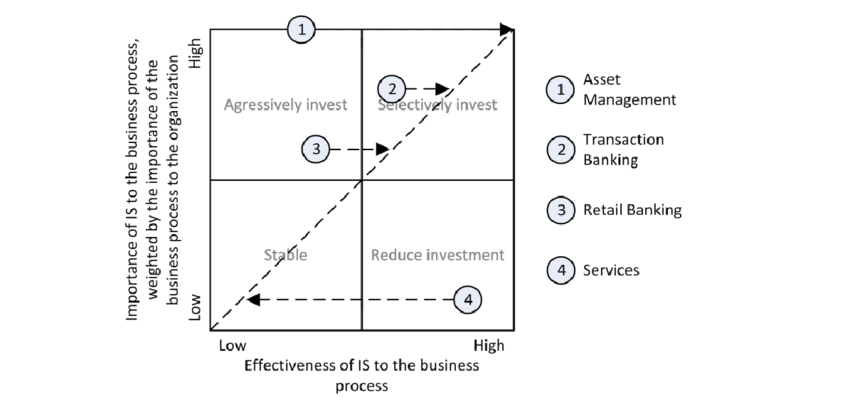
\includegraphics[width=0.8\textwidth]{Content/Cơ sở lý thuyết/documents/Process portfolio/images/ProcessPortfolioIllustration.png}
        \vspace{0.5cm}
        \caption{Ví dụ về Danh mục quy trình (Process portfolio)}
        \label{fig: Ví dụ về Danh mục quy trình (Process portfolio)}
    \end{center}
\end{figure}

Process portfolio đề cập tới một lược đồ có nhiệm vụ trực quan hóa những quy trình nghiệp vụ thông qua những tiêu chí được đề ra. Những quy trình được biểu diễn dưới dạng những node, thông tin của từng node sẽ được cung cấp từ phía người dùng và cả từ những đánh giá của hệ thống về mô hình quy trình nghiệp vụ hiện tại.

Process portfolio giúp người quản lý hình dung được mức độ ưu tiên giữa những quy trình nghiệp vụ, đây là cơ sở để chúng ta có được những bước đi kế tiếp liên quan tới việc phân tích, đánh giá, tái thiết kế quy trình.